\chapter{System Design and Architecture for Dysarthric Speech Recognition}

Designing a robust speech recognition system for dysarthric speech requires careful consideration of data variability, model adaptation, and contextual correction. The system must handle distorted acoustic signals while maintaining meaningful transcription accuracy. This chapter presents the design specifications, modeling choices, and architecture of the proposed hybrid pipeline. It also details the methodology and design considerations involved in integrating ASR, synthetic data generation, and semantic correction mechanisms.

\section{Specifications for the Design}

The system is designed with the following specifications:
\begin{itemize}
\item Input: Dysarthric speech audio (real, augmented, or synthetic)
\item Output: Corrected text transcription
\item Model: Whisper-based ASR with parameter-efficient fine-tuning
\item Processing: On-device or local inference for privacy preservation
\item Robustness: Ability to handle noise and speech variability
\item Evaluation: Performance measured using Word Error Rate (WER) and Character Error Rate (CER)
\end{itemize}

\section{Pre-analysis and Model Selection}

The design begins with evaluating existing ASR models and identifying their limitations for dysarthric speech. Whisper is selected due to its robustness across diverse audio conditions. However, its performance degrades on impaired speech due to distribution mismatch.

To address this, the following components are incorporated:
\begin{itemize}
\item Synthetic speech generation using TTS and voice conversion
\item Noise augmentation for real-world robustness
\item Parameter-efficient fine-tuning (LoRA) for domain adaptation
\item Large Language Models (LLMs) for semantic correction
\end{itemize}

This combination forms a hybrid architecture that improves both acoustic and semantic understanding.

\section{Design Methodology}

The proposed system follows a multi-stage pipeline:

\begin{enumerate}
\item \textbf{Data Preparation:} Collection of dysarthric speech datasets and generation of synthetic data using TTS and voice conversion techniques
\item \textbf{Data Augmentation:} Application of noise injection, pitch shifting, and tempo variations to simulate real-world conditions
\item \textbf{Feature Extraction:} Conversion of audio signals into log-Mel spectrograms using Whisper’s feature extractor
\item \textbf{Model Adaptation:} Fine-tuning Whisper using LoRA to adapt to dysarthric speech patterns
\item \textbf{Decoding:} Generating initial transcription using beam search decoding
\item \textbf{Semantic Repair:} Using a local LLM and Personal Knowledge Graph to correct transcription errors
\end{enumerate}

This structured pipeline ensures robustness at both acoustic and semantic levels.

\begin{figure}[H]
	\centering
	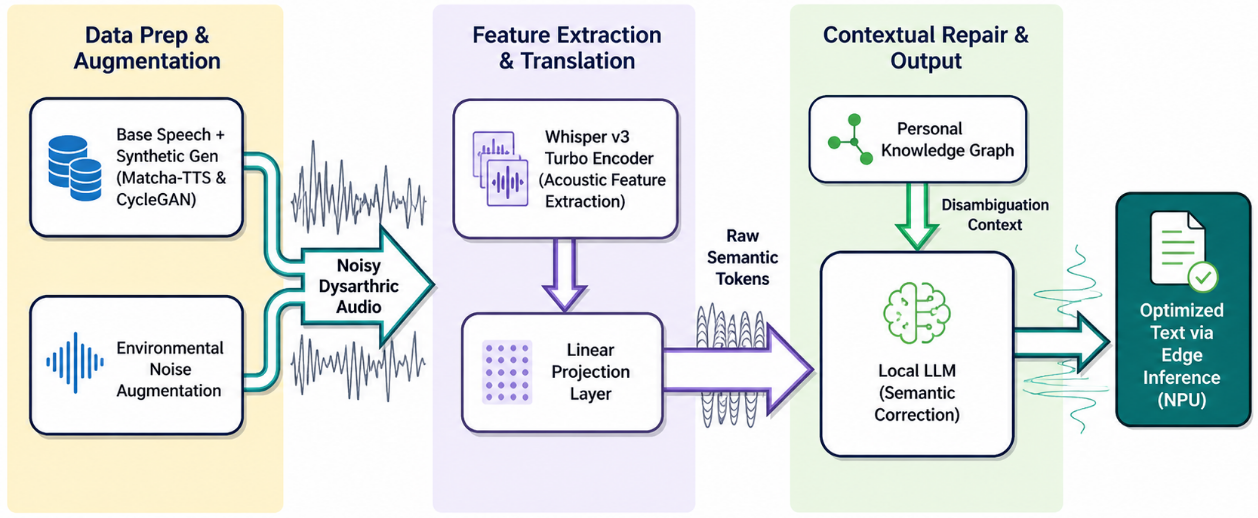
\includegraphics[width=1.0\textwidth]{Figures/system_pipeline_flow.png}
	\caption{System Pipeline Flow}
	\label{fig:system_pipeline}
\end{figure}

\begin{figure}[H]
	\centering
	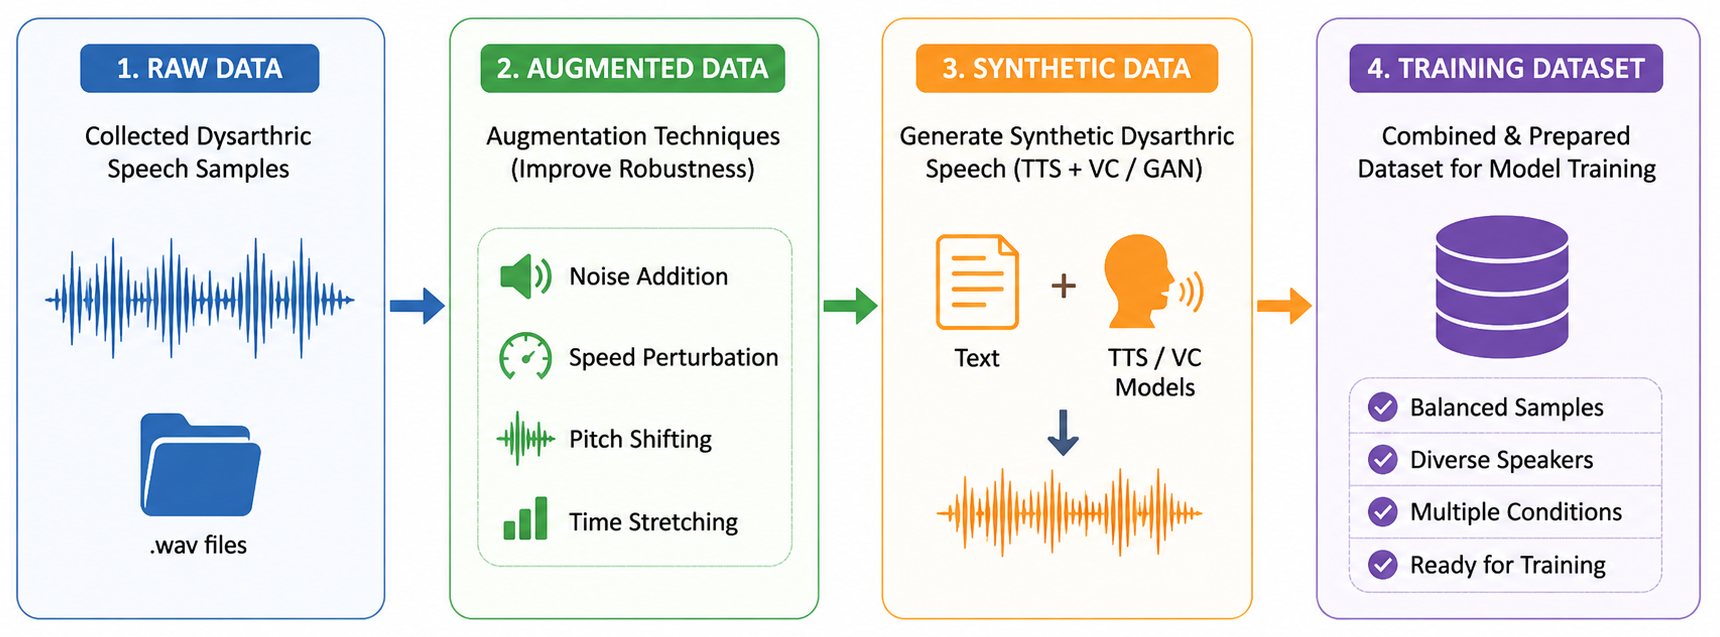
\includegraphics[width=1.0\textwidth]{Figures/data_pipeline_augmentation.png}
	\caption{Data Pipeline}
	\label{fig:data_pipeline}
\end{figure}

\begin{figure}[H]
	\centering
	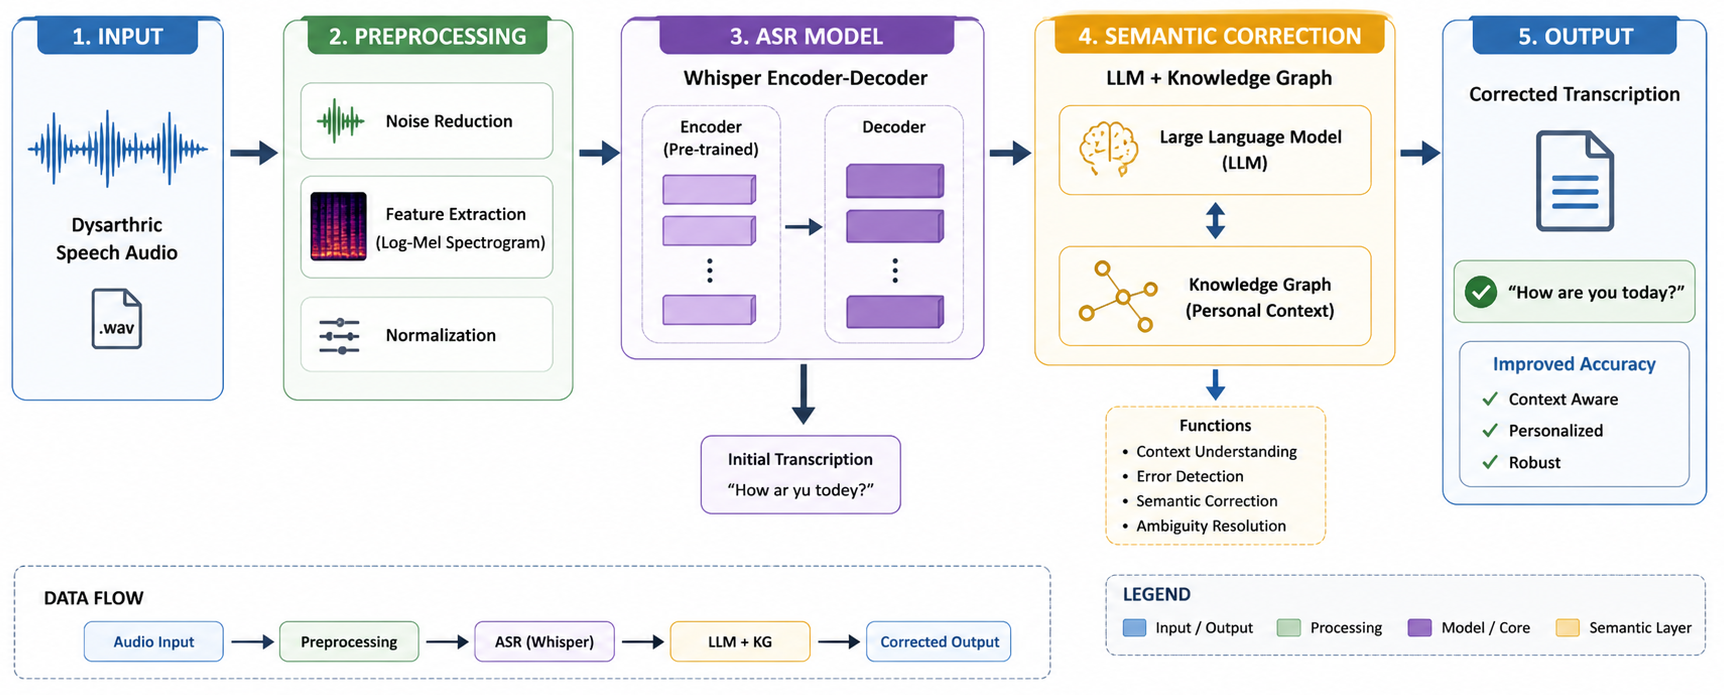
\includegraphics[width=0.9\textwidth]{Figures/architecture_block_diagram.png}
	\caption{System Architecture Block Diagram}
	\label{fig:architecture}
\end{figure}

\section{Design Equations}

The evaluation of the system is based on standard ASR metrics.

Word Error Rate (WER) is defined as:
\[
WER = \frac{S + D + I}{N}
\]
where:
\begin{itemize}
\item $S$ = Substitutions
\item $D$ = Deletions
\item $I$ = Insertions
\item $N$ = Total number of words in reference
\end{itemize}

Character Error Rate (CER) is defined as:
\[
CER = \frac{S + D + I}{N}
\]
where the computation is performed at the character level.

\section{Experimental Techniques}

The system is trained and evaluated using:
\begin{itemize}
\item Dataset splitting into training and testing sets
\item Speaker-aware splitting to avoid data leakage
\item Fine-tuning using LoRA for efficient training
\item Evaluation on unseen datasets to test generalization
\item Comparison of baseline and fine-tuned model performance
\end{itemize}

\section{Summary}

This chapter presented the design and architecture of the proposed dysarthric speech recognition system. It outlined the specifications, modeling choices, and methodology used to build a robust pipeline combining ASR and semantic correction. These design principles guide the implementation and experimentation discussed in the next chapter.